\documentclass{article}
\usepackage{graphicx} % Required for inserting images
\graphicspath{{Images/}}
\usepackage[utf8]{inputenc}
\usepackage{multicol}
\usepackage{amsthm}
\usepackage{amsmath}
\usepackage{xcolor}
\usepackage{wrapfig}

\newtheorem{definition}{Definition}[section]
\newtheorem{remark}{Remarque}[section]
\newtheorem{theorem}{Théorème}[section]

\title{Physique : Mécanique}
\author{Laura Paraboschi / Simon Lefort}
\date{BA1-IN}

\begin{document}

\maketitle

\section{Lois de Newton}

\begin{enumerate}
    \item \[ \sum\overrightarrow{F} = \textbf{0} \leftrightarrow MRU \] 
    \item \[ \sum\overrightarrow{F} = m \cdot \overrightarrow{a}  \] 
    \item \[ \overrightarrow{F}_{1 \rightarrow 2} = -\overrightarrow{F} _{2 \rightarrow 1} \]
\end{enumerate}


\section{M.R.U.A}

\[ v(t) = a_ot + v_0 \]
\[ x(t) = \frac{1}{2}a_0t^2 + v_ot + x_o \]

\section{Cinématique du point matériel}
\subsection{Produit scalaire}
\begin{definition}
    Un scalaire est un nombre défini comme :
    \[ \overrightarrow{a}\cdot \overrightarrow{b} = |\overrightarrow{a}||\overrightarrow{b}| \cos{\theta} <=> |\overrightarrow{a}||proj_{\overrightarrow{b}\rightarrow \overrightarrow{a}}| <=> |\overrightarrow{b}||proj_{\overrightarrow{a}\rightarrow \overrightarrow{b}}|\]
    \begin{figure}[h]
        \centering
        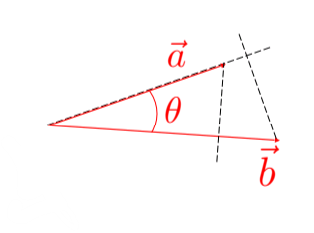
\includegraphics[height=3cm]{Images/Produit scalaire.png}
        \label{fig:prodscal}
    \end{figure}
    \\En composantes (repère orthonormé) :
    \[ \overrightarrow{a} \cdot \overrightarrow{b} =  a_1b_1 + a_2b_2 + a_3b_3\]
    Propriétés :
    \begin{multicols}{2}
        \begin{itemize}
            \item \( \overrightarrow{a} \cdot \overrightarrow{b} = \overrightarrow{b} \cdot \overrightarrow{a} \)
            \item \( \overrightarrow{a} \cdot (\overrightarrow{b} + \overrightarrow{c}) = \overrightarrow{a} \cdot \overrightarrow{b} + \overrightarrow{a} \cdot \overrightarrow{c}\)
            \item \( \overrightarrow{a}  \cdot (\lambda\overrightarrow{b}) = \lambda(\overrightarrow{a} \cdot \overrightarrow{b}) \)
        \end{itemize}
        \columnbreak
        \begin{itemize}
            \item \( \overrightarrow{a} \cdot \overrightarrow{b} = \overrightarrow{0} \) Si les vecteurs sont orthogonaux
            \item \( \overrightarrow{a} \cdot \overrightarrow{a} = |\overrightarrow{a}|^2 \geq 0\)
        \end{itemize}
    \end{multicols}
\end{definition}
\subsection{Projection et composantes d'un vecteur}
Projection sur l'axe û :
\[ \overrightarrow{OP} \cdot \hat{u} = |\overrightarrow{OP}| |\hat{u}|\cos{\theta} = OP\cos{\theta} \]
Coordonnées carthésiennes :
\begin{equation}
    \begin{cases}
        x = \overrightarrow{OP} \cdot \hat{x}\\
        y = \overrightarrow{OP} \cdot \hat{y}\\
        z = \overrightarrow{OP} \cdot \hat{z}
    \end{cases}
\end{equation}
\[ \overrightarrow{OP} = x\hat{x} + y\hat{y} + z\hat{z} = \begin{pmatrix}
    x \\
    y \\
    z
\end{pmatrix} \]
\subsection{Repère direct}
La chiralité est définie par la règle du \textcolor{red}{tire-bouchon} ou de la \textcolor{blue}{main droite}
\begin{wrapfigure}{l}{0.75\textwidth}
    \centering
    \includegraphics[width = 0.75\textwidth]{Images/Repère.png}
    \label{fig:repere}
\end{wrapfigure}
\begin{remark}
En posant le bas du poing contre le "plan" créé par \( \overrightarrow{v}_1, \overrightarrow{v}_2 \), il faut que les doigts s'enroulent de \( \overrightarrow{v}_1 \rightarrow \overrightarrow{v}_2 \). Le sens du pouce indiquera le sens de \( \overrightarrow{v}_3 \)\newline \newline \newline\newline\newline\newline\newline\newline
\end{remark}
\subsection{Produit vectoriel \(\overrightarrow{a} \wedge \overrightarrow{b}\)}
\begin{wrapfigure}{r}{0.3\textwidth}
    \centering
    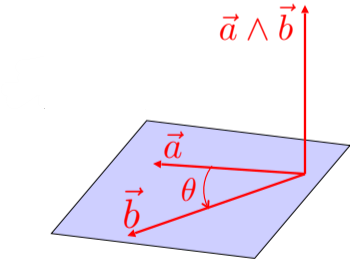
\includegraphics[width = 0.30\textwidth]{Images/Plan.png}
    \label{fig:plan}
\end{wrapfigure}
\begin{definition}
    Vecteur
    \begin{itemize}
        \item direction : normale au plan défini par \( \overrightarrow{a} \) et \( \overrightarrow{b} \) 
        \item sens : règle de la main droite
        \item norme : \( |\overrightarrow{a}||\overrightarrow{b}|\sin{\theta} \)
    \end{itemize}
\end{definition}
En composantes :
\[ \overrightarrow{a} \wedge \overrightarrow{b} = \begin{vmatrix}
    \hat{x}_1 & a_1 & b_1 \\
    \hat{x}_2 & a_2 & b_2 \\
    \hat{x}_3 & a_3 & b_3
\end{vmatrix} = \begin{pmatrix}
    a_2b_3 - a_3b_2 \\
    a_3b_1 - a_1b_3 \\
    a_1b_2 - a_2b_1
\end{pmatrix}\]
Propriétés :
\begin{itemize}
    \item \( \overrightarrow{a} \wedge \overrightarrow{b} = -\overrightarrow{b} \wedge \overrightarrow{a} \)
    \item \( \overrightarrow{a} \wedge (\overrightarrow{b} + \overrightarrow{c}) = \overrightarrow{a} \wedge \overrightarrow{b} + \overrightarrow{a} \wedge \overrightarrow{c} \)
    \item \( \overrightarrow{a} \wedge (\lambda \overrightarrow{b}) = \lambda (\overrightarrow{a} \wedge \overrightarrow{b}) \)
    \item Vecteurs colinéaires : \( \overrightarrow{a} \wedge \overrightarrow{b} = \overrightarrow{0} \)
\end{itemize}
Produit mixte :\\\\
\( (\overrightarrow{a} \wedge \overrightarrow{b}) \cdot \overrightarrow{c} = \begin{vmatrix}
    c_1 & a_1 & b_1 \\
    c_2 & a_2 & b_2 \\
    c_3 & a_3 & b_3
\end{vmatrix} \)\\\\\\
\( (\overrightarrow{a} \wedge \overrightarrow{b}) \cdot \overrightarrow{c} = (\overrightarrow{c} \wedge \overrightarrow{a}) \cdot \overrightarrow{b} = (\overrightarrow{b} \wedge \overrightarrow{c}) \cdot \overrightarrow{a}\) \\\\
\( (\overrightarrow{a} \wedge \overrightarrow{b}) \cdot \overrightarrow{c} = 0 \Leftrightarrow \overrightarrow{a}, \overrightarrow{b} et \overrightarrow{c} coplanaires\)\\\\
Double produit vectoriel :\\\\
\( \overrightarrow{c} \wedge (\overrightarrow{a} \wedge \overrightarrow{b})  = (\overrightarrow{c} \cdot \overrightarrow{b})\overrightarrow{a} - (\overrightarrow{c} \cdot \overrightarrow{a})\overrightarrow{b} \) \\\\
Distributivité de la dérivation :\\\\
\( \frac{d}{dx}(\overrightarrow{a} \cdot \overrightarrow{b}) = (\frac{d\overrightarrow{a}}{dx} \cdot \overrightarrow{b}) + (\overrightarrow{a} \cdot \frac{d\overrightarrow{b}}{dx}) \) \\\\
\( \frac{d}{dx}(\overrightarrow{a} \wedge \overrightarrow{b}) = (\frac{d\overrightarrow{a}}{dx} \wedge \overrightarrow{b}) + (\overrightarrow{a} \wedge \frac{d\overrightarrow{b}}{dx}) \)\\
\subsection{Données sur graphe}
\begin{wrapfigure}{l}{0.5\textwidth}
    \centering
    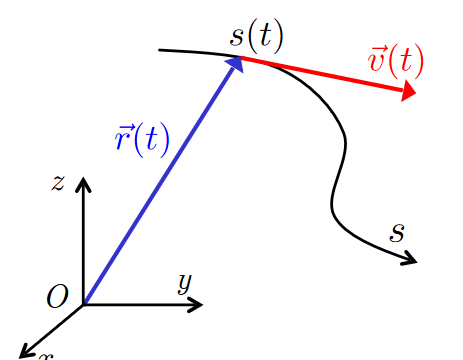
\includegraphics[width=6cm]{Images/Mouvement.png}
    \caption{Cinématique}
    \label{fig:cinématique}
\end{wrapfigure}
\( \overrightarrow{r}(t) = \) Position par rapport à O \\\\
\( \overrightarrow{v}(t) = \frac{d \overrightarrow{r}}{dt} = \) vitesse vectorielle instantanée (tangente à la trajectoire)\\\\
\( s(t) =\) abcisse curviligne = distance parcourue \\\\
\( v(t) = |\overrightarrow{v}(t)| = \) vitesse scalaire \\\\
\( \hat{\tau} = \) vecteur unitaire tangent à la trajectoire\\\\\\\\
\begin{figure}[htp]
    \centering
    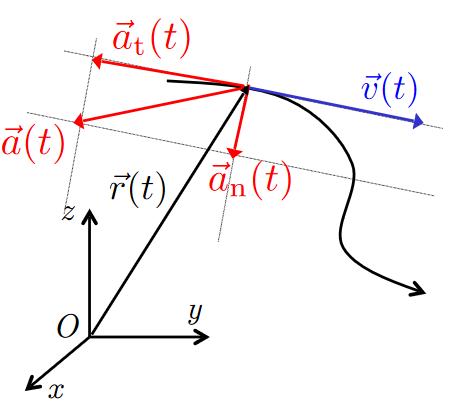
\includegraphics[width=6cm]{Images/acceleration.png}
    \caption{Accélération}
    \label{fig:acceleration}
\end{figure}
\( \overrightarrow{a}(t) = \frac{d\overrightarrow{v}}{dt} = \overrightarrow{a}_t(t) + \overrightarrow{a}_n(t) = \) accélération vectorielle instantanée \\\\
\( \overrightarrow{a}_t(t) = \) accélération tangentielle \\\\
\( \overrightarrow{a}_n(t) = \frac{v^2}{R} = \) accélération normale \\
Traiter \( \overrightarrow{a}_t(t) \) en considérant un MRUA tangent (si acc. tan. constante)
\subsection{Mouvement avec vitesse scalaire constante}
\[ \overrightarrow{F} = m\overrightarrow{a} \Rightarrow F = m\frac{v^2}{R} \] \newpage
\subsection{Système de coordonnées}
\begin{figure}[htp]
    \centering
    \includegraphics[width=12cm]{Images/coordonnées.png}
    \label{fig:coord}
\end{figure}

\subsection{Rotations spatiales}
\begin{figure}[htp]
    \centering
    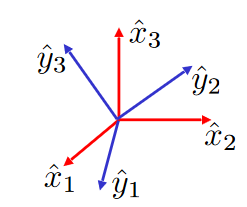
\includegraphics[width = 4cm]{Images/Rotation.png}
    \caption{Rotation d'axe}
    \label{fig:rotation}
\end{figure}
Deux types :
\begin{itemize}
    \item Rotation de l'axe, objet fixe
    \item Rotation de l'objet, axes fixes 
\end{itemize}
\begin{theorem}[Théorème d'Euler]
    Soit deux repères orthonormés droits de même origine : Il existe toujours une rotation qui amène le premier sur le deuxième
\end{theorem} \newpage
\subsection{Repères et vecteur en rotation}
Matrice E :
\(\begin{pmatrix}
    0 & -\omega_3 & \omega_2 \\
    \omega_3 & 0 & \omega_1 \\
    -\omega_2 & \omega_1 & 0
\end{pmatrix} \) \qquad Matrice \(  \overrightarrow{\omega} = \begin{pmatrix}
    \omega_1 \\
    \omega_2 \\
    \omega_3
\end{pmatrix}\) \\\\
Vecteur fixe (repère en rotation) : \[ \frac{d\overrightarrow{r}}{dt} = E\overrightarrow{r} = \overrightarrow{\omega} \wedge \overrightarrow{r} \]\\
Formule de Poisson (vecteur du repère) : \[  \dot{\hat{e}}_i = \frac{d\hat{e}_i}{dt} = \overrightarrow{\omega} \wedge \hat{e}_i \]
\begin{figure}[htp]
    \centering
    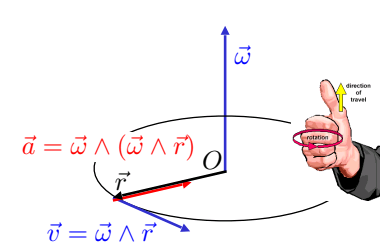
\includegraphics[width=6cm]{Images/vitesse angulaire.png}
    \caption{Vitesse angulaire}
    \label{fig:angu}
\end{figure}
\newline Le vecteur \( \omega \) est parallèle à l'axe de rotation, et son sens est donné par la règle de la main droite
\[ \omega = \frac{d\phi}{dt}\]
Si $\omega$ est constant alors (MCU):
\[ \overrightarrow{v} = \overrightarrow{\omega} \wedge \overrightarrow{r}  \]
\[ \overrightarrow{a} =  \overrightarrow{\omega} \wedge (\overrightarrow{\omega} \wedge \overrightarrow{r}) \] \newpage
\subsection{Vitesse et accélération en coordonnées cylindriques}
\( \overrightarrow{r} = \overrightarrow{OP} = \rho\hat{e}_{\rho} + z\hat{e}_z \) \\
\( \overrightarrow{v} = \dot{\overrightarrow{r}} = \dot{\rho}\hat{e}_{\rho} + \rho\dot{\phi}\hat{e}_{\phi} + \dot{z}\hat{e}_z \) \\
\( \overrightarrow{a} = \ddot{\overrightarrow{r}} = (\ddot{\rho} - \rho\dot{\phi}^2)\hat{e}_{\rho} + (\rho\ddot{\phi} + 2\dot{\rho}\dot{\phi})\hat{e}_{\phi} + \ddot{z}\hat{e}_z \) \\

\[ \overrightarrow{w} = \frac{d\phi}{dt}\hat{z} = \dot{\phi}\hat{z}\]
\begin{figure}[htp]
    \centering
    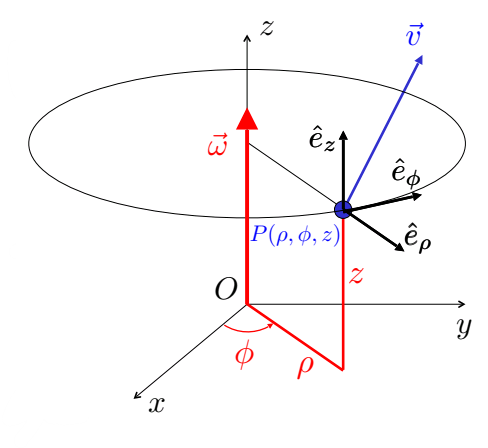
\includegraphics[width=6cm]{Images/MCU.png}
    \caption{Coordonnées cylindriques}
    \label{fig:cylindre}
\end{figure}
\begin{definition}
    La force de liaison est la force exercée sur sur le point matériel pour qu'il obéisse à une contrainte géométrique
    \begin{itemize}
        \item Perpendiculaire à la surface
        \item Jamais de composante tangente à la surface
        \item La force de liaison devient nulle \(\Leftrightarrow\) La contrainte disparait
    \end{itemize}
\end{definition}
\newpage
\subsection{Vitesse et accélération en coordonnées sphériques}
\( \overrightarrow{r} = \overrightarrow{OP} = r\hat{e}_{r}\) \\
\( \overrightarrow{v} = \dot{\overrightarrow{r}} = \dot{r}\hat{e}_{r} + r\dot{\theta}\hat{e}_{\theta} + r\dot{\phi}\sin{\theta}\hat{e}_{\phi} \) \\
\( \overrightarrow{a} = \ddot{\overrightarrow{r}} = (\ddot{r} - r\dot{\theta}^2 - r\dot{\phi}^2 \sin^2{\theta})\hat{e}_{r} + (r\ddot{\theta} + 2\dot{r}\dot{\theta} - r\dot{\phi}^2 \sin{\theta}\cos{\theta})\hat{e}_{\theta} + (r\ddot{\phi}\sin{\theta} + 2\dot{r}\dot{\phi}\sin{\theta} + 2r\dot{\phi}\dot{\theta}\cos{\theta})\hat{e}_{\phi}  \) \\

\[ \overrightarrow{w} = \dot{\phi}\hat{z} + \dot{\theta}\hat{e}_{\phi} \]
\begin{figure}[htp]
    \centering
    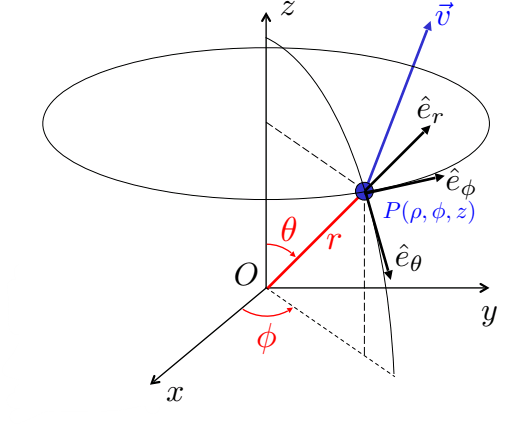
\includegraphics[width=6cm]{Images/spherique.png}
    \caption{Coordonnées sphériques}
    \label{fig:spherique}
\end{figure}

\subsection{Méthode résolution du problème du pendule}

\begin{itemize}
    \item Poser contrainte $ \rho = L \rightarrow \dot{\rho} = 0 \rightarrow \ddot{\rho} = 0  $ 
    \item Poser $ z = 0 \rightarrow \dot{z} = 0 \rightarrow \ddot{z} = 0  $ 
    \item Projeter $ \overrightarrow{P} $ et $ \overrightarrow{T} $ sur $ \hat{e}_{\rho} $ et $ \hat{e}_{\phi} $ 
    \item Poser $ sin(\phi) \approx{\phi} $
    \item Résoudre $ \ddot{\phi} = \frac{-g}{L} \cdot \phi $
\end{itemize}

\end{document}
